\section{Case Study: Competitive Hackathon}
\label{sec:casestudy}

We report on the application of MEP during a competitive hackathon
to illustrate the methodology's behavior under realistic constraints. The
setting imposed fixed time limits, external evaluation, and a requirement to
produce working software---conditions that favor rapid iteration and
penalize unproductive preparation.

\subsection{Setting}

The hackathon took place in January 2026, organized around a publisher's
editorial archive and an AI-powered content API. Approximately 12 teams
competed in a five-hour window to build working prototypes, with judging
by an industry panel and a \$5{,}000 prize for the top project. Teams
self-organized around pitches submitted before the event~\cite{event2026hackathon}.
The practitioner-researcher had professional backgrounds in both
education and software engineering, a combination that informed the
product concept and design decisions throughout the event.

\subsection{Preparation Phase}

While most teams began coding within the first fifteen minutes, the
practitioner-researcher spent approximately two hours in deliberate
preparation, applying the three phases described in
Section~\ref{sec:methodology}.

\textbf{Contextual grounding} produced 10 planning documents totaling 9,386
words, including API exploration notes, competitive analysis, and---critically---an
extended dictation on pedagogical design philosophy drawn from the practitioner's
teaching experience, encoding tacit knowledge about how effective learning
environments create conditions for student thinking~\cite{polanyi1966tacit}.

\textbf{Collaborative specification} occurred concurrently, as the practitioner
refined the product concept through dialogue with an AI agent. The resulting
specification described a platform where teachers curate bounded research
environments from The Atlantic's archive and students conduct research using a
Socratic AI tutor. Key value judgments encoded in the specification included
constraining the product to a single assignment type (prioritizing depth over
breadth for a three-minute demo),
insisting on real API data rather than mocks, and scoping the analytics dashboard
to show the student's research \emph{journey} rather than only the final submission.

\textbf{Task decomposition} converted the specification into 64 structured
task records with priorities and dependencies. The planning-to-code
ratio---9,386 words of planning against 8,496 lines of source code---was
1.10:1. Table~\ref{tab:timeline} summarizes the timeline alongside the
deployment commit cadence.

\begin{table}[t]
  \centering
  \caption{Hackathon timeline, artifacts, and deployment cadence. Phases
    overlap inside the preparation block; agent implementation runs in
    parallel across four agents. The deployment-and-polish window
    produces nine commits at $\sim$5~minute mean intervals.}
  \label{tab:timeline}
  \footnotesize
  \begin{tabular}{@{}lrl@{}}
    \toprule
    \textbf{Phase} & \textbf{Duration} & \textbf{Key Artifacts / Cadence} \\
    \midrule
    Contextual grounding   & $\sim$2 hr      & 10 docs (9,386 words) \\
    Collab.\ specification & (concurrent)    & Product specification \\
    Task decomposition     & (concurrent)    & 64 beads w/ dependencies \\
    Agent implementation   & 184 min         & 43 beads closed (med.\ 5.9 min) \\
    \midrule
    Deploy: setup        & 22:24--22:39    & 5 commits, 1 every 3 min \\
    Deploy: gap          & 22:39--22:49    & --- \\
    Deploy: content fixes & 22:49--23:17    & 4 commits, 1 every 7 min \\
    \bottomrule
  \end{tabular}
\end{table}

\subsection{Implementation and Results}

Four parallel subagents were deployed across distinct feature areas:
classroom creation, student research workspace, day-one/\allowbreak
day-thirty demo toggle, and Socratic AI tutor. The agents drew on the
contextual grounding documents and specification produced during
preparation. The 64 task records served as the interface between
preparation and execution (Figure~\ref{fig:methodology}); each bead
encoded an independently executable unit with boundaries that required
no inter-agent coordination. Closure timestamps confirm genuine
parallelism: agents completed work simultaneously across feature
areas, with a median closure time of 5.9~minutes per bead
(Figure~\ref{fig:beadtimes}). The subsequent deployment phase produced
9~commits over 52~minutes. The final codebase comprised 43
TypeScript/TSX files totaling 8,496 lines, deployed to production as a
full-stack educational platform.

\begin{figure}[t]
  \centering
  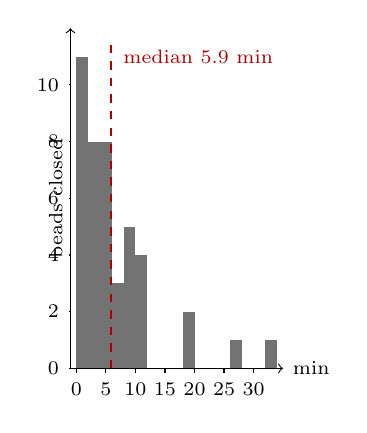
\begin{tikzpicture}[
    yscale=0.36, xscale=0.075,
    every node/.style={font=\scriptsize},
  ]
    %% Axes
    \draw[->] (-1,0) -- (35,0) node[right, font=\scriptsize] {min};
    \draw[->] (-1,0) -- (-1,12);
    %% x ticks
    \foreach \x in {0,5,10,15,20,25,30}
      \draw (\x,0) -- (\x,-0.18) node[below, font=\scriptsize] {\x};
    %% y ticks (counts)
    \foreach \y/\lab in {0/0,2/2,4/4,6/6,8/8,10/10}
      \draw (-1,\y) -- (-1.3,\y) node[left, font=\scriptsize] {\lab};
    %% Histogram bars: 2-min bins of closure times for n=43 beads
    %% Bins (lower, count): [0,2):11, [2,4):8, [4,6):8, [6,8):3,
    %%   [8,10):5, [10,12):4, [12,14):0, [14,16):0, [16,18):0,
    %%   [18,20):2, [20,22):0, [22,24):0, [24,26):0, [26,28):1,
    %%   [28,30):0, [30,32):0, [32,34):1
    \fill[black!55] (0,0)  rectangle (2,11);
    \fill[black!55] (2,0)  rectangle (4,8);
    \fill[black!55] (4,0)  rectangle (6,8);
    \fill[black!55] (6,0)  rectangle (8,3);
    \fill[black!55] (8,0)  rectangle (10,5);
    \fill[black!55] (10,0) rectangle (12,4);
    \fill[black!55] (18,0) rectangle (20,2);
    \fill[black!55] (26,0) rectangle (28,1);
    \fill[black!55] (32,0) rectangle (34,1);
    %% median line
    \draw[dashed, thick, red!70!black] (5.9,0) -- (5.9,11.6);
    \node[red!70!black, anchor=west, font=\scriptsize] at (6.3,11) {median 5.9 min};
    %% y label
    \node[rotate=90, font=\scriptsize] at (-3.5,6) {beads closed};
  \end{tikzpicture}
  \caption{Per-bead completion time distribution across the 43 closed
    hackathon beads. Most work units complete inside a single 10-minute
    agent session; long-tail outliers correspond to API-client and
    state-persistence tasks executed in parallel with shorter
    decomposed work.}
  \label{fig:beadtimes}
\end{figure}

Three observations bear on evaluation. First, the architecture required no
structural refactoring during deployment: the bugs that emerged were
integration and styling issues (API content truncation, inter-component
data flow, favicon configuration), not architectural misalignment.
Second, the preparation-to-execution ratio was approximately 5.7:1
(two hours of preparation against $\sim$21 minutes of active
implementation per agent across four parallel agents). Bug-type beads
resolved at a median 1.2~minutes (mean 1.5~min) versus 9.7~minutes for
implementation tasks, suggesting parallel-execution defects were
detected and corrected quickly.
Third, near-zero architectural rework is consistent with the hypothesis
that rich upfront context reduces agent misalignment, though we cannot
establish causation from a single case study.

\subsection{Variation Across Teams}
\label{sec:teamvariation}

The 12-team field offers a qualitative sketch of how peers approached
the same constraints. We did not instrument other teams; identities are
anonymized and observations are coarse-grained, drawing on publicly
shared pitches and event observation. Table~\ref{tab:teams} groups
pitches into thematic clusters with each team's described workflow style.

\begin{table}[t]
  \centering
  \caption{Twelve-team field at the hackathon, grouped by problem
    cluster, with workflow style as inferred from pitches and
    observation. Identifiers are anonymized; ``vibe'' denotes a
    self-described non-technical or iterative-prompting workflow,
    ``decomp.'' denotes explicit planning before coding, and ``mixed''
    denotes both modes within one team.}
  \label{tab:teams}
  \scriptsize
  \begin{tabular}{@{}p{0.06\columnwidth}p{0.46\columnwidth}p{0.16\columnwidth}p{0.12\columnwidth}@{}}
    \toprule
    \textbf{ID} & \textbf{Pitch theme} & \textbf{Cluster} & \textbf{Workflow} \\
    \midrule
    T1  & Infinite-canvas archive graph        & Discovery       & decomp.\ \\
    T2  & Reading-comprehension overlay        & Education       & vibe \\
    T3  & In-article excerpt exploration       & Discovery       & mixed \\
    T4  & AI ``knowledge gauge'' (reading level) & Accessibility & vibe \\
    T5  & Auto-generated event timelines       & Context         & vibe \\
    T6  & Topic-following / catch-up alerts    & Personalization & mixed \\
    T7  & Editorial content optimization (CORE) & Personalization & decomp.\ \\
    T8  & Reader-interpretation probes         & Trust           & decomp.\ \\
    T9  & Structured reader-expert input       & Trust           & decomp.\ \\
    T10 & Argument-evolution interaction layer & Discovery       & decomp.\ \\
    T11 & Newsroom knowledge-graph copilot     & Productivity    & decomp.\ \\
    T12 & Curated classroom research workspace (this study) & Education & decomp.\ \\
    \bottomrule
  \end{tabular}
\end{table}

Three patterns emerge. \textbf{Workflow style} split roughly in half:
teams whose pitch flagged a non-technical author or vibe-coding intent
(T2, T4, T5) leaned on iterative prompting, while engineering-led teams
(T1, T7--T12) opened with explicit planning artifacts before
generating code. \textbf{Single- versus multi-agent} use trended toward
single-agent loops; only T12 (this study) explicitly fanned out
parallel subagents from a decomposed plan. \textbf{Artifact production}
was correspondingly uneven: vibe-leaning teams presented working
surfaces with limited written specification, whereas
decomposition-leaning teams produced design notes shared with judges.
We cannot link these patterns to outcome quality without controlled
comparison, but the field reads as a natural sample of the
preparation-versus-iteration spectrum that motivates RQ1 and the
multi-team replication study in Section~\ref{sec:agenda}.
